\documentclass[runningheads,svgnames]{llncs}
%
\usepackage[]{graphicx}
\usepackage{amsmath}
\usepackage{hyperref}
\usepackage{cleveref}
% \usepackage{tikz}
% \usepackage{nth}
% \usepackage{subcaption}
\usepackage{booktabs}
% \usepackage{array}
\usepackage{orcidlink}
\usepackage{subcaption} % Addition
\usepackage{multirow} % Addition
\usepackage{tabularx} % Addition
\usepackage{booktabs} % Addition
\usepackage{siunitx} % Addition
\usepackage{scalerel}
\usepackage{cleveref}


% \usetikzlibrary{shadings,decorations,decorations.pathreplacing}
\renewcommand\UrlFont{\color{blue}\rmfamily}
% FIXME proper hyperref setup

\newcommand{\mcite}[1]{\text{\cite{#1}}}
\newcommand{\mref}[1]{\text{\ref{#1}}}

% \renewcommand{\baselinestretch}{0.97}


% Comment 
% FIXME : delete before submission :)
\newcommand{\bertrand}[1]{\textcolor{violet}{Bertrand:~#1}}
\newcommand{\nathalie}[1]{\textcolor{purple}{Nathalie:~#1}}
\newcommand{\edwin}[1]{\textcolor{pink}{Edwin:~#1}}
\newcommand{\joseph}[1]{\textcolor{red}{Joseph:~#1}}

% Customize table rendering
\setlength{\tabcolsep}{5pt}
\renewcommand{\arraystretch}{1.4}

\begin{document}
%
\title{A Benchmark of Named Entity Recognition Approaches in Historical Documents\\
Application to 19$^{th}$ Century French Directories%
% FIXME "19$^{th}$-Century" with dash?
% \thanks{%
% This work was supported by the French National Research Agency:
% Project SoDuCo, grant ANR-18-CE38-0013.% ???FIXME need acknowledgments for directory sources???
% }
}
%
\titlerunning{A Benchmark of NER Approaches in Historical Documents}
%
\author{%
N. Abadie\inst{1}\orcidlink{0000-0001-8741-2398} \and
E. Carlinet\inst{2}\orcidlink{0000-0001-5737-5266} \and
J. Chazalon\inst{2}\orcidlink{0000-0002-3757-074X} \and
B. Duménieu\inst{3}\orcidlink{0000-0002-2517-2058}\\
{\footnotesize \emph{all authors contributed equally}}%
}
%
\authorrunning{N. Abadie et al.}
%
\institute{%
% 1
LASTIG, Univ. Gustave Eiffel, IGN-ENSG, F-94160 Saint-Mandé, France\\
\email{nathalie-f.abadie@ign.fr}%\\
% \url{https://www.umr-lastig.fr/nathalie-abadie/}%
\and
% 2
EPITA Research \& Development Laboratory (LRDE), Le Kremlin-Bicêtre, France\\
\email{\{edwin.carlinet,joseph.chazalon\}@lrde.epita.fr}%\\
%\url{https://lrde.epita.fr}
\and
% 3
CRH-EHESS, Paris, France\\
\email{bertrand.dumenieu@ehess.fr}%\\
% \url{http://crh.ehess.fr/index.php?5206}\\
\joseph{Je propose de supprimer les URLs.}%
}
%
\maketitle              % typeset the header of the contribution
%
\begin{abstract}
% !TeX root = ../main-paper.tex
Named entity recognition (NER) is a necessary step in many pipelines targeting historical documents.
Indeed, such natural language processing techniques identify which class each text token belongs to,
e.g. ``person name'', ``location'', ``number''.
Introducing a new public dataset built from 19th century French directories,
we first assess how noisy modern, off-the-shelf OCR are.
Then, we compare modern CNN- and Transformer-based NER techniques
which can be reasonably used in the context of historical document analysis.
We measure their requirements in terms of training data,
the effects of OCR noise on their performance,
and show how Transformer-based NER can benefit from unsupervised pre-training 
and supervised fine-tuning on noisy data (\cref{fig.pipeline-overview}).
Results can be reproduced using resources available at \url{https://github.com/soduco/paper-ner-bench-das22}.
% The latest version of is paper can be obtained at \url{https://arxiv.org/abs/xxxx.xxxxx}.
\keywords{Historical documents \and Natural Language Processing \and Named Entity Recognition \and OCR noise \and Annotation cost.}
\end{abstract}

% ---- Sections ----
% !TeX root = ../main-paper.tex
\begin{figure}[!h]
    \centering
    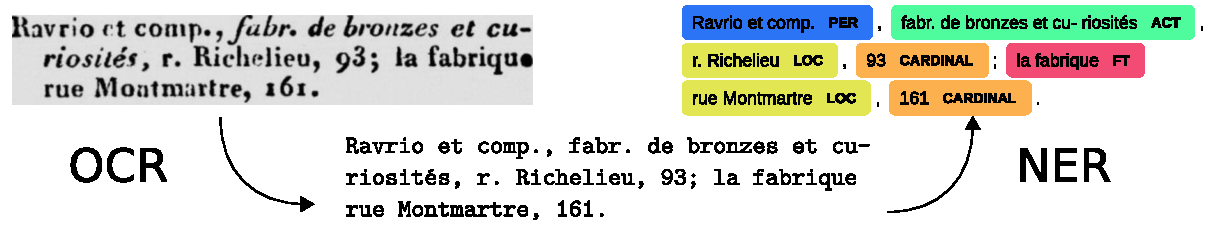
\includegraphics[width=.9\textwidth]{figs/overview-intro.pdf}
    \caption{%
    Overview of the pipeline under study.
    From previously-extracted images of directory entries, 
    we perform OCR and named entity recognition (NER) using different techniques.
    We aim at answering the following questions:
    \emph{How noisy are modern, out-of-the-box OCR systems?}
    \emph{What is the behaviour of NER when OCR is noisy?}
    \emph{Can NER be made more robust to OCR noise?}
    }
    \label{<label>}
\end{figure}
\clearpage% force float flush!

\section{Introduction}

% General context + scope limitation
OCRed texts are generally not sufficient to build a high level semantic view of a collection of historical documents.
A subsequent stage is often needed to extract the pieces of information most likely to be searched for by users, such as named entities: persons, organisations, dates, places, etc.
Indeed, being able to properly tag text tokens unlocks the ability to relate entities and provide colleagues from other fields with databases ready for exploitation.

Being active research topics, OCR and named entity recognition (NER) are still difficult tasks when applied to historical text documents.
OCR approaches used for modern documents are likely to struggle even on printed historical documents due to multiple causes related to text readability (low resolution scans, inconsistent printing rules, artefacts, show-through), document complexity (intricate and versatile page layout, use of ancient fonts \& special glyphs) and the variability inherent to the great diversity of historical sources.
On the other hand, the semantics of entities in NER approaches developed for modern texts may be different from those in ancient texts.

In this article, we focus on a corpus of printed trade directories of Paris from the XIX\textsuperscript{th} century, containing hundreds of pages long lists of people with their activity and address.
They provide fine-grained knowledge to study the social dynamics of the city over time.
As they originate from different publishers, they show a diversity in layout, information organisation and printing quality, which adds to the poor digitising quality to make OCR and NER challenging tasks.

Trade directories have been leveraged in a recent work to identify polluted urban soils \cite{bell2020automated} and locate all gas stations in the city of Providence over the last century.
In an ongoing research project we aim at producing structured spatio-temporal data from the entries in the Paris trade directories to study the transformations of the fraction of XIX\textsuperscript{th} century Parisian society reachable through these sources.
%Because they originate from several publishers, their content is organised following different indexing methods (by name, by activity or by address), is printed in various layouts, and uses different fonts.
Therefor, we investigate several state-of-the-art OCR and NER approaches to assess their usability to process the corpus.

The contributions of this article are the following.
% Contributions
\begin{enumerate*}[(i)]
    \item We review state of the art OCR and NER systems for historical documents (\cref{sec:related-work}).
    \item We introduce a new dataset suitable for OCR and NER evaluation (\cref{sec:dataset}).
    \item We measure the performance of three modern OCR systems on real data (\cref{sec:ocr-xp}).
    \item We evaluate modern NER approaches: their requirements in terms of training data, and the effects of pre-training (\cref{sec:ner-xp1}).
    \item We show that Transformed-based NER can benefit from pre-training and fine-tuning to improve its performance on noisy OCR (\cref{sec:ner-xp2}).
\end{enumerate*}



% !TeX root = ../main-paper.tex
\section{OCR and NER on historical texts}
\label{sec:related-work}

\joseph{Suggestion pour réduire la présentation de l'état de l'art : l'orienter exclusivement vers une justification des systèmes que nous avons retenus pour cet article.}

The directory processing pipeline presented in \cite{bell2020automated} includes an OCR step, done with Tesseract, and a NER step to identify company names and addresses, performed using regular expressions.
This section reviews existing OCR and NER approaches with historical texts and presents some works assessing the effects of OCR quality on the NER performance and the proposed solutions. 

\subsection{Optical Character Recognition on historical texts}

Most of the current state-of-the-art OCR systems, like Tesseract \cite{smith2007overview}, OCRopus \cite{breuel2008ocropus} and PERO OCR \cite{kohut2021ts} are based on a pipeline of convolutional neural networks (CNNs) and long short-term memory networks (LSTM).
Although this kind of model produces good results with modern texts, it faces several challenges with ancient texts, such as the lack of annotated data for learning, or different transcription styles in training data.

\cite{martinek2019hybrid} propose an approach to generate synthetic annotated text for historical OCR training, based on manually collected characters from historical text images.
This work proposes to train an OCR system based on a CNN-LSTM network with synthetic data and then to fine-tune the model with some pages of real historical annotated text.
The results show that this approach gives state-of-the-art results. 

To overcome the limitations due to different transcription styles in training data, PERO OCR adds a Transcription Style Block layer to a classical model based on a CNN and a Recurrent Neural Network components \cite{kohut2021ts}.
This block takes the image of the text and a Transcription Style Identifier as inputs and helps the network decide what kind of transcription style to use as output.

\joseph{Move to implementation details for XP OCR or to pipeline summary}
\begin{itemize}
    \item Tesseract 4.1.1 (newest version: 5, released Nov. 2021)
    \item Pero OCR version from git repo, master branch updated on Sep 15, 2021 % 8b20f29    
    \item other?  % kraken if times allows
\end{itemize}


% PERO refs
% O Kodym, M Hradiš: Page Layout Analysis System for Unconstrained Historic Documents. ICDAR, 2021.
% M Kišš, K Beneš, M Hradiš: AT-ST: Self-Training Adaptation Strategy for OCR in Domains with Limited Transcriptions. ICDAR, 2021.
% J Kohút, M Hradiš: TS-Net: OCR Trained to Switch Between Text Transcription Styles. ICDAR, 2021.


\subsection{Named Entity Recognition}

Many approaches have been designed to recognize named entities, ranging from handcrafted rules to supervised approaches \cite{nadeau2007}.
Rule based approaches look for portions of the text that match patterns like in \cite{bell2020automated,nouvel2011} or dictionary (gazetteers, author lists, etc.) entries like in \cite{mansouri2008,maurel2011}.
Such kind of approaches achieve very good results when applied to a specialized domain corpus and when an exhaustive lexicon are available, but at high system engineering cost \cite{nadeau2007}. 

Supervised approaches include both approaches implementing supervised learning algorithms with careful text feature engineering, and deep learning based approaches which automatically build their own features to classify tokens into named entity categories.
In recent years, the latter have grown dramatically, yielding state-of-the-art performances as shown in the recent survey proposed by \cite{li2020}. This survey concludes that fine-tuning general-purpose contextualized language models with domain-specific data is very likely to give good performance for use cases with domain-specific texts and few training data. This strategy has been adopted by \cite{Labusch2020NamedED} to extract named entities in OCRed historical texts in German, French, and English. However, the NER performance decreased dramatically with OCRed texts is noted, especially for the English texts for which the OCR is of poorer quality. 

\subsection{Improving Named Entity Recognition in historical texts}
\label{subsection:stoa-ner-on-historical-texts}


Several recent studies have focused on the extent to which the quality of the OCR affects the results produced by a NER model.
\cite{van2020assessing} assess the impact of OCR on several NLP downstream tasks, including NER. They worked on a corpus published by a post-OCR correction software company, made of many journal articles with different levels of OCR errors and their respective ground truths.
For each OCRed article, the Word Error Rate (WER) is computed and the English model \textit{en-core-web-lg} provided by Spacy\footnote{\url{https://spacy.io/}} library is used to perform NER on \textit{Person}, \textit{GPE}\footnote{Geopolitical Entity} and \textit{Date}.
The performance of the NER model with respect to OCR quality is eventually assessed by computing the F-measure for each NER class, and each article i.e., each WER value.
\cite{hamdi2020assessing} performed a similar but more extensive evaluation on four different NER models: CoreNLP using Conditional Random Fields and three deep neural models, BLSTM-CNN, BLSTM-CRF, and BLSTM-CNN-CRF.
They tested them on two well-known NER benchmark corpora: CoNLL-02 and CoNLL-03. They applied four different types of OCR noise to each corpus, with two levels of degradation and computed the WER and Character Error Rate (CER) for each degraded version.
Finally, they applied each NER model to the progressively degraded versions of the corpus and computed the resulting F-measure.
Overall, NER F-measure drops from 90\% to 50\% when the WER increase from 8\% to 50\%. However, models based on deep neural networks seem less sensitive to OCR errors.

\cite{huynh2020use} and \cite{marz2021data} have proposed different approaches to reduce the negative impact of OCR errors on NER performance with historical texts.
The former uses a spelling correction tool on several corpora with variable OCR error rates, to assess whether NER performance benefit from spelling corrections or not.
As long as OCR errors remain low (CER<2\% and WER<10\%), the F-measure of NER results remains stable.
It starts to decrease significantly when OCR errors exceed these thresholds.
The latter work focuses on adapting the training data to facilitate the generalization of an off-the-shelf NER model from modern texts to historical texts.
Three different NER models are tested on three historical corpora, in French, English, and Dutch. The best results are produced by a model trained on clean modern data, including embeddings computed with Flair on a historical corpus, and fine-tuned on a noisy historical ground truth.

In conclusion, NER approaches based on deep learning seem to be more suitable for dealing with historical texts as they adapt more easily to OCR errors than rule-based approaches.
Recent work in this area suggests that the impact of OCR quality on NER can be reduced by using different strategies.
On the one hand, if the OCR error rate is kept below a certain threshold, the NER models remain little impacted: it is therefore important to reduce OCR errors as much as possible, but a low error rate may remain acceptable.
On the other hand, reusing a NER model trained on modern data and adapted to historical texts using supervised or unsupervised approaches seems a good strategy. 




\subsection{== À réintégrer depuis ancienne section 4 ==}
We select two deep-learning-based NER models available in packaged software libraries: SpaCy NLP pipelines and CamemBERT.


\subsubsection{spacy}
Spacy is a software library that offers NLP components assembled in modular pipelines specialised by language.
Although BERT is available in the latest version of SpaCy (v3), the pipeline for French does not provide a NER layer at the time of our experiments (jan. 2022).
Hence, we rely on SpaCy's ad hoc pipeline trained on French corpora and capable of named entity recognition.
% deep-sequoia and wikiner-fr, capable of named entity recognition.\textit{fr\_core\_news\_lg}\footnote{https://spacy.io/models/fr} trained two corpora in French: deep-sequoia and wikiner-fr, capable of named entity recognition.
The global architecture of these pipelines have not been yet published but are explained by the developers on their website.
Words are first encoded into local context-aware embeddings using a window-based CNN similar to~\cite{collobert2011}.
The decision layer is an adaptation of the transition-based model presented in~\cite{lample2016}.
As words are processed sequentially, their vectors are concatenated with those of the last known entities to encode the nearby predicted semantics.
The classification layer relies on a finite-state machine whose transition probabilities are learned using a multilayer perceptron.
% \bertrand{Drop the next sentences if we need space}
% In 2018~\cite{won2018} evaluated SpaCy's NER ability to detect place names in five corpora of ancient letters written in English.
% They measured an average F1 score of 0.57.
% The SpaCy developers claim an accuracy of 0.85 for the English NER pipeline \textit{en\_core\_web\_lg} on the OntoNotes 5.0 corpus\footnote{https://spacy.io/usage/facts-figures}.
%For our experiments, the French model \textit{fr\_core\_news\_lg} is fine-tuned using our ground truth corpus.


% Other possibilities:
%1. Traditional ML based:
%    Conditional Random Fields (CRF) - https://pypi.org/project/sklearn-crfsuite/
%    Maximum-entropy Markov model

%2. Neural Networks based:
%    LSTMs, bi-LSTM - https://github.com/flairNLP/flair
%    CNNs (SpaCy uses CNN based architecture)
%    Transformers (Spacy has recently launched it) - %https://spacy.io/universe/project/spacy-transformers


\subsubsection{Transformers / Bert / Hugging face}
Language model based on \textit{Transformers} \cite{vaswani2017attention}, like BERT \cite{devlin2018bert}, have become a new paradigm for NER\cite{li2020}. 
The learned embeddings can be used as distributed representations for input instead of traditional embeddings like Google Word2Vec, and they can be further fine-tuned for NER by adding an additional output layer. 
They can also be pretrained in an unsupervised way on historical texts for domain adaptation.
As the directories are written in French, we chose the language model CamemBERT \cite{martin-etal-2020-camembert}, a Transformer model trained on a French corpus.
\joseph{plutôt tourner ça pour dire qu'il existe des modèles FR / qu'on est limités par la dispo de modèles FR pré-entraînés ?}

\subsection{Pipeline summary}

\Cref{fig.protocol} depicts the evaluation protocol used to assess the OCR and NER systems. 

\begin{figure}[tb]
    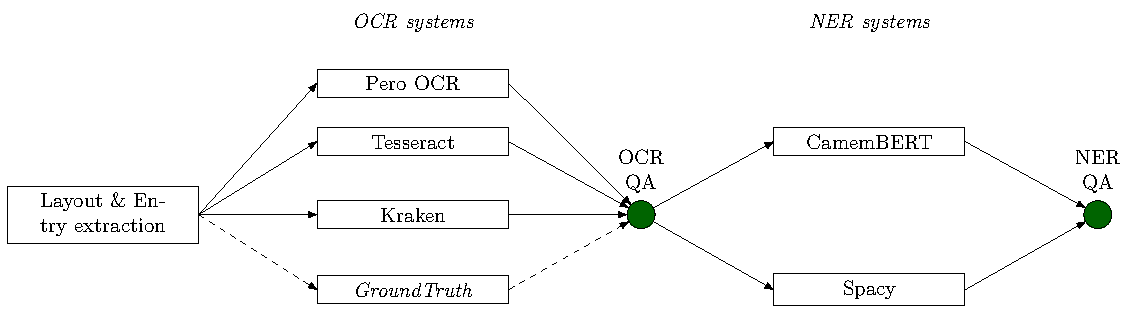
\includegraphics[width=\linewidth]{figs/protocol.pdf}
    \caption{Scheme of the evaluation protocol. \joseph{Missing "Ground truth" for NER stage?}}
    \label{fig.protocol}
    \end{figure}



% !TeX root = ../main-paper.tex
\section{Dataset}

% !TeX root = ../main-paper.tex
\section{NER Approaches}

Previous work on the influence of OCR errors on NER models shows that it is preferable to reuse a model trained on modern data and adapt it to OCRised historical texts using supervised or unsupervised approaches. This is why, in our tests, we have selected two deep learning-based NER approaches trained on French texts: Spacy 3 NER pipeline and CamemBERT. 

\subsubsection{Regexp}
::TODO::
Needed for experiment 2 ?

\subsubsection{Spacy 3 NER pipeline}
The \textit{of the shelf} NLP library SpaCY offers a named entity recognition tool based on an ad hoc architecture which has not been yet published but is explained by the developers on their website. Although the latest version of SpaCy (v3) leverages BERT models, we could not use them as no NER pipeline is available for the French language at the time of our experiments\footnote{https://spacy.io/models/fr}.
The vanilla NER pipeline is two-fold. Words are first encoded into local context-aware embeddings using a window-based CNN similar to~\cite{collobert2011}.
The decision layer is an adaptation of the transition-based model presented in~\cite{lample2016}.
As words are processed sequentially, their vectors are concatenated with those of the last known entities to encode the nearby predicted semantics as a dynamic attention mechanism.
The classification layer relies on a finite-state machine whose transition probabilities are learned using a multilayer perceptron.
In 2018~\cite{won2018} compared SpaCy's vanilla NER performance on historical texts about places with several other software packages (Stanford-NER, Ner-Tagger, Edinburgh Geopoarser and Polyglot). Results showed SpaCy to be average with a F1-score of 0.57.
The SpaCy developers claimed an accuracy of 0.85 for the English NER pipeline \textit{en\_core\_web\_lg} on the OntoNotes 5.0 corpus\footnote{https://spacy.io/usage/facts-figures}.

\subsubsection{CamemBERT \& CamemBERT+pretrained on raw entries}
::TODO::

Language model embeddings pretrained using Transformers, like BERT, have become a new paradigm for NER\cite{li2020}. Indeed, these embeddings can be used as distributed representations for input instead of traditional embeddings like Google Word2Vec and they can be further fine-tuned for NER task by adding an additional output layer. Moreover, they can also be further pretrained in an unsupervised way on historical texts for domain adaptation.

As our directories are written in French, we chose the language model CamemBERT \cite{martin-etal-2020-camembert}, a Transformer model trained on a French corpus. We started from the CamemBERT-ner model already fine-tuned on WikiNER-fr corpus and published on the Hugging Face repository \footnote{\url{https://huggingface.co/Jean-Baptiste/camembert-ner}}. Its output layer is a linear model with a Softmax function.

For our experiments, two models are derived. One is produced by fine-tuning this generic model on our ground truth dataset.
The second is created by adapting the embeddings of this model using raw directory texts, randomly selected and extracted with PERO OCR. The base model is pretrained on these texts for two tasks, namely, Next Sentence Prediction (NSP) and Masked Language Model (MLM). Finally, the resulting model is also fine-tuned using our ground truth corpus.

% Other possibilities:
%1. Traditional ML based:
%    Conditional Random Fields (CRF) - https://pypi.org/project/sklearn-crfsuite/
%    Maximum-entropy Markov model

%2. Neural Networks based:
%    LSTMs, bi-LSTM - https://github.com/flairNLP/flair
%    CNNs (SpaCy uses CNN based architecture)
%    Transformers (Spacy has recently launched it) - %https://spacy.io/universe/project/spacy-transformers
% !TeX root = ../main-paper.tex
\section{Experimental Setup}


\begin{figure}[tb]
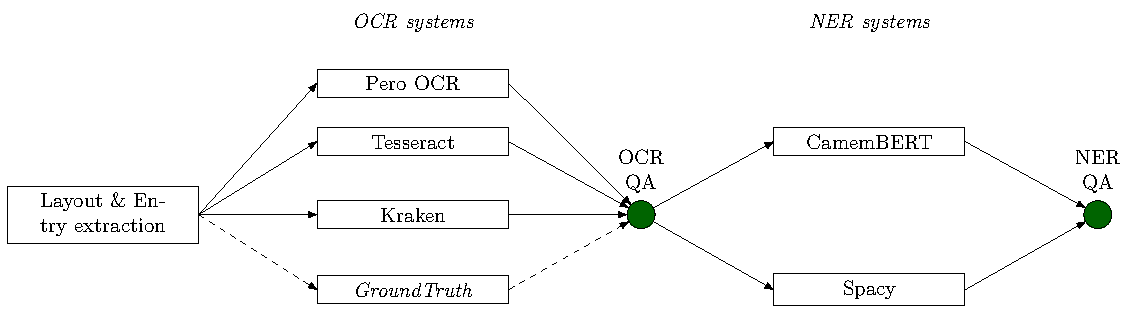
\includegraphics[width=\linewidth]{figs/protocol.pdf}
\caption{Scheme of the evaluation protocol. \joseph{Missing "Ground truth" for NER stage?}}
\label{fig.protocol}
\end{figure}

\subsection{Evaluation protocol \& Metrics}

The Figure \Cref{fig.protocol} depicts the evaluation protocol used to assess the OCR and NER systems. Two quality evaluations
are performed in the pipeline, respectively named \emph{OCR Q.A.} and \emph{NER Q.A.}.

First, the layout extraction and entry segmentation of the page are performed with a semi-automated system and
checked by a human. Afterward, an OCR system runs on the thumbnails of each segmented entry to extract its text. An
entry might span over multiple text lines but is always a single block. Thus, the most adapted mode is chosen when
the OCR system allows for the detection mode (e.g. the \emph{block} mode for \emph{Tesseract}). 

\textbf{OCR Q.A.} is performed after some text normalization of the OCR system outputs. Text normalization consists in
projecting Unicode characters onto the latin-1 charset (whenever it makes sense) and removing extra symbols (hands,
crosses). Then, the predicted text is aligned with the reference text using standard tools and the Character Error Rates
(CER) are computed at the entry level and at the global level. 

\begin{align}
\mathrm{CER} &=  \frac{\#Errors}{\text{Reference Text Length}} & & \mathrm{CER}_\mathrm{norm} =  \frac{\#Errors}{\text{Alignment Length}} 
\end{align}

In this benchmark, we consider 3 OCR systems well known for historical document analysis: Pero OCR, Tesseract, and Kraken. 

\edwin{FIXME: add ref papier eval OCR + ISRI, eval KRAKEN}


Next, a NER system extracts the named entities from the text of each entry output by the OCR and the \textbf{NER Q.A.}
is performed. The NER system outputs a text with tags that enclose the entities. To assess the quality of the entity
extraction, we rely on a technique similar as for the OCR evaluation. The predicted text is aligned with the reference
text and the tags are projected in the alignment. Then, the precision, recall, and f-measure (or f-score) are computed considering
only the exact matches between entities. Precision and recall are defined by equation (2); the f-measure is their harmonic mean.

\begin{align}
    \mathrm{precision} &= \frac{\text{\#exact matches}}{\text{\#entries in prediction}} & \mathrm{recall} &= \frac{\text{\#exact matches}}{\text{\#entries in reference}}
\end{align}


The whole process is illustrated on~\cref{fig.eval-ocr-ner}. The OCR text and the GOLD text are first aligned to
evaluate the OCR accuracy. As there are 11 mismatches over 56 aligned characters, the CER is thus 24\%. This alignment
is then used to back-project the GOLD tags to build the tagged NER reference string. Finally, the NER system runs on the
OCR text; its output is compared to the NER reference string. There is only 2 over 3 tags matching in the prediction (precision),
while only 2 over 4 entities are matched in the reference (recall). It follows an overall f-score of 0.4.

\begin{figure}[tb]
    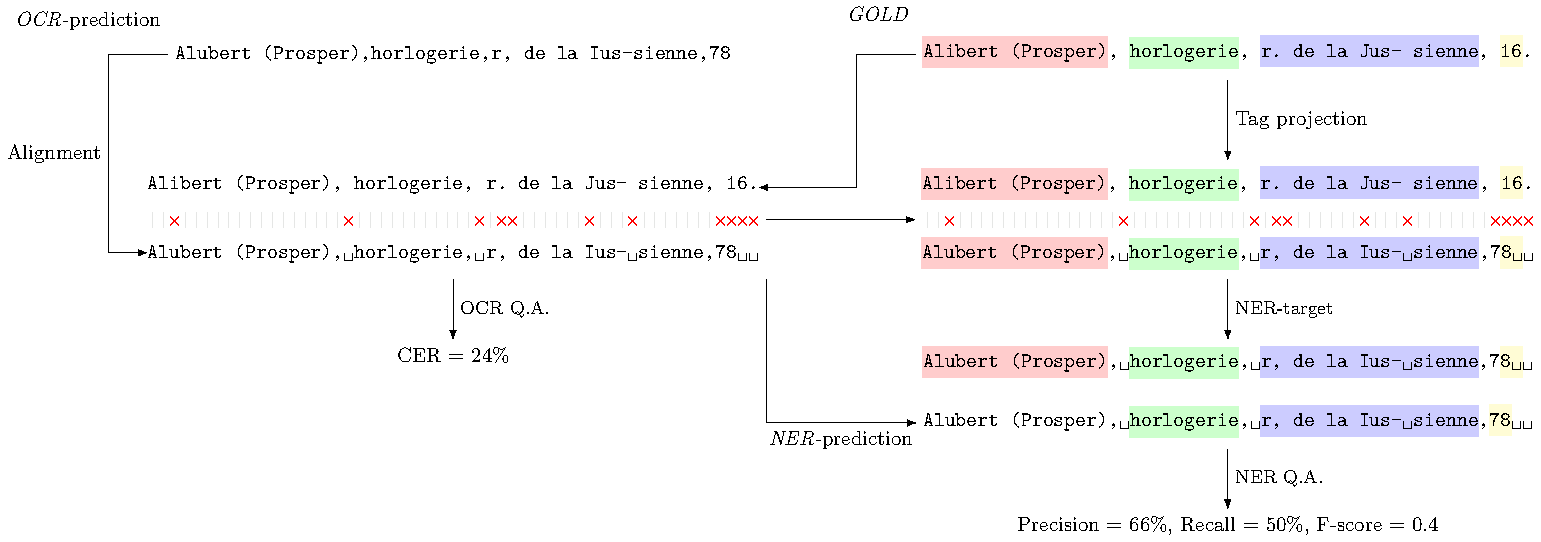
\includegraphics[width=\linewidth]{figs/eval-ocr-ner.pdf}
    \label{fig.eval-ocr-ner}
    \caption{OCR and NER evaluation protocol example.}
\end{figure}


\subsection{Experiment 1: NER sensibility to the number of training examples}
\label{subsection:experiment-1-setup}
\bertrand{Find a better name ?}
The constitution of annotated example sets to train a NER model on a target domain a is a critical preliminary step.
Often done manually, possibly from bootstrapped annotations, this task is tedious, time consuming and error prone.
The ability of a model to perform well even with few training examples is a pratical criteria to consider.
In this first experiment, we investigate the performance of the three models when fine-tuned for NER on training sets of decreasing sizes.

To do so, we split the gold reference of manually annotated entries into a training set, a development set, and a test set. 
The training set is then gradually reduced in size while maintaining the relative frequency of directories within it.

As the organisation and structure of entries varies across directories, the models may learn to overfit on a subset of directories with specific features.
To reduce the evaluation bias, we start by leaving out 3 directories (1690 entries, $\approx 19\%$) from the gold reference to test each model on unseen directories.
Then, a stratified sampling based on the source directory of each entry is run on the remaining set to create a training (6373 entries, $\approx 73\%$ of the gold reference) and a development set (709 entries, $\approx 8\%$).
This sampling procedure is a convenient way to shape both sets so they reflect the diversity of directories within the gold reference.
The development set is used to evaluate the models performance during the training phase.
To generate smaller training sets, we start from the initial training set and iteratively split it in half using the same stratified sampling strategy as before.
We stop if a directory has only one entry left, or if the current training subset contains less than 30 entries.
Applying this procedure to the initial training set produced 8 training subsets containing 49, 99, 199, 398, 796, 1593, 3186, and 6373 entries.

All tree models are fine-tuned for NER on each training subset.
The performance metrics are measured against the test set after each training.


% Move to results
%All metrics are evaluated on the test set, yet the biased metrics on the development set are added in the article material as additional information.


\subsection{Experiment 2: Impact of OCR nosie on named entity recognition}
\label{subsection:experiment-2-setup}
Noise introduced by OCR is known to impede the named entity recognition process (see section~\ref{subsection:stoa-ner-on-historical-texts}).
%The second experiment assesses the impact of the OCR on the quality of the NER results.
The second experiment addresses two questions (1) which model is the most robust to OCR noise and (2) what is the most appropriate strategy to fine-tune the NER layer if the input texts to label are noisy ?
To this end, we leverage the labeled OCR datasets produced following to the method explained in Section 5, in addition to the gold reference.

First and foremost, to make sure that the datasets contain the same entries a preprocessing step must be performed.
Indeed, entries where the OCR produced an empty string and those for which no entity could be projected from the gold reference text are ignored.
To overcome this problem we filter each dataset by keeping only the entries common to all.
At the cost of losing  5\% of the gold references entries, we thus have four new annotated datasets containing the exact same entries.
They are denoted hereafter {reference, pero, tesseract}-gold.
Finally each is is split into a training, a dev and a test subset following the procedure presented in\cref{subsection:experiment-1-setup}.

We fine-tune CmBERT and CmBERT+ptrn on reference-gold and pero-gold to create two versions of each model: the former trained on manually corrected entries and the latter on OCR entries.
SpaCy NER is left aside as results from experiment 1 show that it is outperformed by BERT models.
Performance metrics are computed for each of the four resulting NER models against the test sets created from reference-gold, pero-gold and tesseract-gold.

\subsection{Implementation details}

\subsubsection{OCR system parameters}
\nathalie{Y a-t-il des précisions à ajouter sur la façon dont ont été utilisés les OCR? Ou bien ce sont les versions "sur étagère" qui ont servi?}
\joseph{Totalement sur l'étagère. On a normalisé un peu les données après, c'est tout.}
\begin{itemize}
    \item Tesseract 4.1.1 (newest version: 5, released Nov. 2021)
    \item Pero OCR version from git repo, master branch updated on Sep 15, 2021 % 8b20f29    
    \item other?  % kraken if times allows
\end{itemize}

Pero OCR uses ParseNet \joseph{TODO ref} as internal layout parser for line detection.
Pero OCR uses an LSTM engine \joseph{TODO check + ref} for text line recognition.
Pero OCR generally works very well, as long as the bounding boxes of the regions to recognize are not too tightly adjusted.
Trained on newspapers in European languages by its development team.
Can output results in Latin, Greek and Cyrillic scripts, as well as some commonly-used typographic symbols.

% PERO refs
% O Kodym, M Hradiš: Page Layout Analysis System for Unconstrained Historic Documents. ICDAR, 2021.
% M Kišš, K Beneš, M Hradiš: AT-ST: Self-Training Adaptation Strategy for OCR in Domains with Limited Transcriptions. ICDAR, 2021.
% J Kohút, M Hradiš: TS-Net: OCR Trained to Switch Between Text Transcription Styles. ICDAR, 2021.


\subsubsection{Spacy}
We use the French pipeline \textit{fr\_core\_news\_lg} provided by SpaCy v.3.2.1\mcite{spacy}, already trained for NER on the deep-sequoia and wikiner-fr corpora.
The default NER labels known to the pipeline are PER, ORG, MISC and LOC.
In experiment 1 the base model is fine-tuned on every of the 8 training sets using the same training parameters.
Early stopping is activated with a patience value of 1600 training steps without improvement of the f1 score.


% \bertrand{Move to results}
%For each size of the training dataset, 5 runs are performed, always with the same parameters, and the mean value of each performance score is computed.

%library and leverage the library utilities to fine-tune it on various training and validation datasets derived from our ground truth dataset (see Section 5.2 for details). The base model is fine-tuned in turn on each of the 8 generated training datasets, using the same training parameters. Early stopping is activated with patience parameters set at 1600. For each size of the training dataset, 5 runs are performed, always with the same parameters, and the mean value of each performance score is computed.

%and Huggingface for the BERT 
%tok2vec(words embeddings + encoding) + attention layer  +  transition-based %model.

\subsubsection{Huggingface CamemBERT}
Experiments 1 and 2 rely on the implementation of transformers provided by the software library Huggingface (transformers v.4.15.0, datasets v.1.17.0).
Our baseline CmBERT model is CamemBERT model published on the Hugging Face repository \footnote{\url{https://huggingface.co/Jean-Baptiste/camembert-ner}} and already trained for NER on wikiner-fr.
Its NER head is a linear model with a Softmax function.
CmBERT and CmBERT+ptrn are always fine-tuned using the same parameters, with at most 5000 training steps and an early stopping condition set to 3 evaluations in experiment 1 (5 in experiment 2) without improvement of the f1 score. Evaluations are performed every 100 steps.


Details can be found for both the SpaCy NER and the CamemBERT NER models in the source code publicly available on the GitHub repository \bertrand{LIEN GITHUB}.

%$BERT_{reference}$ The base model is fine-tuned in turn on each of the training datasets generated from the groundtruth corpus. Training parameters are set depending on the considered experiment: early stopping is activated with the patience parameter set at 3 for experiment 1 and at 5 for experiment 2.

%$BERT_{pero-ocr}$ This model is used for experiment 2 only. The base model is fine-tuned on the training dataset generated by projecting the named entity annotations on the text extracted by PERO OCR, using the same parameters as for the $BERT_{reference}$ model.

%$BERT_{ptrn-reference}$ The base model is pretrained using 845000 entries extracted by PERO OCR with the Next  Sentence  Prediction  (NSP) and  Masked  Language  Model(MLM) tasks. Then it is fine-tuned with the same parameters and on the same training datasets generated from the groundtruth corpus as the $BERT_{reference}$ model.

%$BERT_{ptrn-pero-ocr}$ This model is used for experiment 2 only. The base model is pretrained like the $BERT_{ptrn-reference}$ model and it is fine-tuned with the same parameters and on the same training datasets as the $BERT_{pero-ocr}$ model.


% !TeX root = ../main-paper.tex
\section{Results}

\subsection{Experiment 1: Accuracy vs NER approach vs training set size}

Qualitative results
\textbf{TODO random samples of results + selection of failure cases}


Quantitative results: table + graph ideally (with training set size info)

\begin{verbatim}
Accuracy
|                             ..o   
|                ..o       o/       
|            ./`          /`          
|        ./o`      .o   o            
|     ./`        .`                    One curve per approach
|    o       o/`                  o  
|          .`                  ./    
|       o`                    /      
|                         .o        
|                       .`           
|                      o            
|                                   
+------------------------------   Training set size
\end{verbatim}
                                        

\subsection{Experiment 2: sensibility to training on noisy data}
Idea : 

Measure : M


\subsection{Experiment 3: Accuracy vs NER approach vs OCR noise}

Qualitative results
\textbf{TODO random samples of results + selection of failure cases}

Quantitative results: table + graph ideally (with OCR noise, same format as previous)

Opt. use synthetic text perturbation as well? Maybe not interesting and too artificial if we have access to 2+ OCR systems.
(original OCR from BNF, Tesseract 4, Pero OCR…)


\subsection{Discussion}
Interesting points to discuss:
\begin{itemize}
    \item can we train on noisy data? (without manual OCR correction?) => future work? cf Pero OCR training procedure?
    \item do we need better OCR systems or better post-correction techniques (if NER is reliable enough)?
    \item Construction of the lexicon and associated cost
\end{itemize}

% !TeX root = ../main-paper.tex
\section{Conclusion and future works}
We assessed the performance of three modern OCR systems on a set of historical sources of great interest in social history.
Although \peroocr clearly outperforms its competitors, the qualitative analysis of OCR errors shows that its failure cases are not the same as Tesseract.
This calls for leveraging both OCR systems in a complementary way to get the best of the two worlds.
%Moreover, we evaluate two deep-learning-based NER approaches in terms of their sensibility to the amount of training data and to noisy OCR texts.
The evaluation of SpaCy NER and CamemBERT (with and without pre-training) showed that BERT-based NER can benefit from pre-training and fine-tuning on a corpus produced with the same process as the texts to annotate.
%However, the results are not as good as for clean text: it is therefore interesting to investigate how to improve the OCR results or to correct the text in a postprocessing step.
Furthermore, it seems that all three models achieve good performance with relatively few training examples.
With a F1-score of 92\% with only 49 training examples, the pre-trained CamemBERT model is a good choice to serve as a bootstrapping model to quickly produce large training sets and therefore lower the burden of creating a ground truth from scratch.
Besides, as directory entries always have the same structure - at least within a given index - we could take advantage of NER results and some simple rules to identify entries within pages instead of relying on the page layout only, or even interactively generate per-index NER models to take advantage of the low amount of training samples required.
We plan to further explore the robustness of the considered NER models by introducing realistic OCR noise in order to identify possible critical points, in terms of noise level or in terms of entities or structural elements affected.

%Interesting points to discuss:
%\begin{itemize}
%    \item can we train on noisy data? (without manual OCR correction?) => future work? cf Pero OCR training procedure?
%    \item do we need better OCR systems or better post-correction techniques (if NER is reliable enough)?
%    \item Construction of the lexicon and associated cost \nathalie{là je ne comprends pas}
%\end{itemize}
%Ideas for future work:
%\begin{itemize}
%    \item Evaluate this: fine-tune Spacy NER on a few samples to generated a bootstrap dataset, feed it to BERT (cleaned or raw) to create an good model with minimal efforts ? \nathalie{les résultats de la table 2 ne plaident pas vraiment pour ça: même sur les très petits corpus, spacy est tours derrière...}
%    \item Use ML to infer regexes ?
%    \item As directories entries are always structured the same way (in a given list at least): use NER to identify entries within pages to save the burden of having to rely on the page layout ?
%\end{itemize}

\section*{Acknowledgments}
This work is supported by the French National Research Agency (ANR), as part of the SODUCO project, under Grant ANR-18-CE38-0013.

The authors want to thank Stéphane Bacciochi and Pascal Cristofoli for helping to create the gold reference dataset, 
Laureencia Maurice for annotating data,
as well as Guillaume Thomas, Paul Abi Saad, Raphaël Lelièvre, Dorian Mignon, Thibault Cavaciuti and Pierre Sadki for contributing to the annotation platform.
\joseph{On peut essayer de gagner de la place en déplaçant ça en footnote de 1ere page.}

% ---- Bibliography ----
\bibliographystyle{splncs04}
\bibliography{ref}
\end{document}
